\documentclass[10pt,landscape]{article}
\usepackage{listings}
\usepackage{multicol}
\usepackage{calc}
\usepackage{mathtools}
\mathtoolsset{showonlyrefs} 
\usepackage{ifthen}
\usepackage[landscape]{geometry}
\usepackage{hyperref}
\usepackage{textcomp}
\usepackage{enumitem}
\usepackage{graphicx}

% To make this come out properly in landscape mode, do one of the following
% 1.
%  pdflatex latexsheet.tex
%
% 2.
%  latex latexsheet.tex
%  dvips -P pdf  -t landscape latexsheet.dvi
%  ps2pdf latexsheet.ps


% If you're reading this, be prepared for confusion.  Making this was
% a learning experience for me, and it shows.  Much of the placement
% was hacked in; if you make it better, let me know...


% 2008-04
% Changed page margin code to use the geometry package. Also added code for
% conditional page margins, depending on paper size. Thanks to Uwe Ziegenhagen
% for the suggestions.

% 2006-08
% Made changes based on suggestions from Gene Cooperman. <gene at ccs.neu.edu>


% To Do:
% \listoffigures \listoftables
% \setcounter{secnumdepth}{0}


% This sets page margins to .5 inch if using letter paper, and to 1cm
% if using A4 paper. (This probably isn't strictly necessary.)
% If using another size paper, use default 1cm margins.
\ifthenelse{\lengthtest { \paperwidth = 11in}}
	{ \geometry{top=.5in,left=.5in,right=.5in,bottom=.5in} }
	{\ifthenelse{ \lengthtest{ \paperwidth = 297mm}}
		{\geometry{top=1cm,left=1cm,right=1cm,bottom=1cm} }
		{\geometry{top=1cm,left=1cm,right=1cm,bottom=1cm} }
	}

% Turn off header and footer
\pagestyle{empty}
 

% Redefine section commands to use less space
\makeatletter
\renewcommand{\section}{\@startsection{section}{1}{0mm}%
                                {-1ex plus -.5ex minus -.2ex}%
                                {0.5ex plus .2ex}%
                                {\normalfont\large\bfseries}}
\renewcommand{\subsection}{\@startsection{subsection}{2}{0mm}%
                                {-1explus -.5ex minus -.2ex}%
                                {0.5ex plus .2ex}%
                                {\normalfont\normalsize\bfseries}}
\renewcommand{\subsubsection}{\@startsection{subsubsection}{3}{0mm}%
                                {-1ex plus -.5ex minus -.2ex}%
                                {1ex plus .2ex}%
                                {\normalfont\small\bfseries}}
\makeatother

% Define BibTeX command
\def\BibTeX{{\rm B\kern-.05em{\sc i\kern-.025em b}\kern-.08em
    T\kern-.1667em\lower.7ex\hbox{E}\kern-.125emX}}

% Don't print section numbers
\setcounter{secnumdepth}{0}


\setlength{\parindent}{0pt}
\setlength{\parskip}{0pt plus 0.5ex}


% -----------------------------------------------------------------------

\begin{document}

\raggedright
\footnotesize
\begin{multicols}{3}


% multicol parameters
% These lengths are set only within the two main columns
%\setlength{\columnseprule}{0.25pt}
\setlength{\premulticols}{1pt}
\setlength{\postmulticols}{1pt}
\setlength{\multicolsep}{1pt}
\setlength{\columnsep}{2pt}

\begin{center}
     \Large{EECS 370 Final Cheat Sheet} \\
\end{center}
\section{ISA}
\begin{itemize}
\item \verb!RISC! : Reduced instruction set computing
\item \verb!CISC! : Complex instruction set computing
\end{itemize}
ARM, MIPS \& LC2K are both RISC. All RISC instructions have the same length (eg: 32-bits for LC2K).
Intel x86 has CISC interface, with RISC core.
\subsection{MIPS}
\begin{tabular}{@{}ll@{}}
\verb!add $s1, $s2, $s3! & \verb!$s1! = \verb!$s2! + \verb!$s3! \\
\verb!beq $s1, $s2, 25! & if(\verb!$s1!==\verb!$s2!) pc=pc+4+100 \\
\verb!lw $s1, 20($s2)! & \verb!$s1! = \verb!Memory![\verb!$s2! + 20] \\
\verb!lui $s1, 20! & \verb!$s1=20*216! \\
\end{tabular} \\
Sign extend if signed, and loading half-word or byte.
If 0x100 = 00, 0x101 = FF, lbu \$s1, 100(\$s0), then \$s1 = 0x000000FF.
\subsection{LC2K}
\begin{tabular}{@{}ll@{}}
\verb!add regA regB destReg!    & \verb!destReg!=\verb!regA!+\verb!regB! \\
\verb!nor regA regB destReg!  & \verb!destReg!=nor(\verb!regA!, \verb!regB!) \\
\verb!lw regA regB field!  & \verb!regB! =*(\verb!regA!+\verb!offset!) \\
\verb!sw regA regB offset!  & *(\verb!regA!+\verb!offset!)=\verb!regB! \\
\verb!beq regA regB offset!  & if(\verb!regA!==\verb!regB!)\verb!pc!+=(\verb!offset!+1) \\
\verb!jalr regA regB!  & \verb!regB!=\verb!pc!+1;\verb!pc!=\verb!regA!; \\
\verb!halt!  & stop program \\
\verb!noop!  & nothing \\
\end{tabular} \\
\subsection{Endianess}
\begin{itemize}
  \item Big-endian: most significant bits stored first
  \item Little-endian: least significant bits stored first
\end{itemize}
\subsection{Two's complement}
Most significant bit is negative, all else is positive.
\begin{equation}
\begin{aligned}
10000001_{\textmd{two}} &= -1 \cdot 2 ^ 7 + 1 = -127 \\
00000001_{\textmd{two}} &= -1 \cdot 2 ^ 0 + 1 = 1 \\
\end{aligned}
\end{equation}
To switch signs, invert and add 1. Also assume unlimited sign extension of most significant bit (eg: $1001_{\textmd{two}} = \cdots 111001_{\textmd{two}}$)
\section{C to Assembly}
\subsection{Memory layout}
\subsubsection{Golden rule}
Address of variable is aligned based on size of the variable.
\begin{itemize}
\item \verb!char! is byte aligned (any addr)
\item \verb!short! is half-word aligned (least significant bit == 0)
\item \verb!int! is word aligned (two least significant bit == 0)
\item \verb!pointer! is size of computer's architecture
\end{itemize}
\subsubsection{Structs}
\begin{itemize}
\item starting addr \% \verb!size(largest basic type)! == 0
\item size \% \verb!size(largest basic type)! == 0
\item allows array of structs
\end{itemize}
\begin{lstlisting}[language=C]
struct record {
  float a;      //0-3
  char b;       //4-4, 5-7 padding
  struct {
    char ** c;  //8-11
    short d[3]; //12-17, 18-19 padding
  } s;          //8-19, 12 % 4 == 0
                //19-23 padding
  double e;     //24-31
  short * f;    //32-35, 37-39 padding
};              //0-39, 40 % 8 == 0
\end{lstlisting}
\subsubsection{Function calls}
Pushed \& poped on call-frame stack in following order:
\begin{enumerate}
  \item incoming params
  \item \$fp
  \item return address
  \item callee saved registers (don't save if not needed)
  \item local vars
  \item spilled registers (when not enough registers)
  \item caller saved registers (don't save dead variables)
  \item outgoing parameters
  \item \$sp
\end{enumerate}
\subsubsection{Liveness example}
\begin{lstlisting}[language=C]
int bar(void) {
  int d = 9;    // d: dead,
  printf("1");  //    overwrite on line 4
  d = 5;        // d: alive
  int e = d;    // e: alive
  printf("2");
  return d + e; // d,e: dead
}
\end{lstlisting}
\subsubsection{Initialization example}
\begin{lstlisting}[language=C]
int g = 0;               // g: static
void bar(int p, int q) { // bar: text
  return p + q;          // p, q: stack
}
int foo() {              // foo: text
  int a = 0;             // a: stack
  static int b = 1;      // b: static
  void (*func_ptr)(int, int) = &bar;
  // func_ptr: stack
  // *func_ptr: text (points to function)
  int *b_ptr = &b;
  // b_ptr: stack
  // *b_ptr: static (points to global)
  static int *m_ptr = malloc(sizeof(int));
  // m_ptr: stack
  // *m_ptr: heap (dynamic allocated)
  return a;
}
\end{lstlisting}
\subsubsection{Translation}
\begin{tabular}{@{}ll@{}}
\verb!header!    & size of other parts \\
\verb!text!  & machine code \\
\verb!data!  & globals \& statics \\
\verb!symbol table!  & symbols \& values \\
\verb!relocation table!  & references to variable addresses \\
\verb!debug info (optional)!  & map to source code \\
\end{tabular} \\
\verb!data! does not contain uninitialized data, but keeps track of how much is needed. \\
\verb!symbol table! contains: \\
\begin{itemize}
\item stuff other files need (globals \& funcs defined in this file)
\item stuff you need (referenced globals \& funcs in this file defined elsewhere)
\item static variables
\end{itemize}
\verb!relocation table! contains: \\
\begin{itemize}
\item address the moved instruction
\item type of instruction (lw, sw, jal, etc)
\item referenced symbol
\end{itemize}
\begin{lstlisting}[language=C,numbers=left]
int brown_dog = 656;
short black_dog = 343;
extern void play_fetch(void);
extern int my_dog_age;

int main() {
  if(my_dog_age == 0)
    static int squirrel = 0;
  my_dog_age = black_dog;
  int i = 0;
  while(i < 3) {
    play_fetch();
    I++;
  }

  int dog_treat = 3;
  int dog_treat_bag = dog_treat * 55;
  my_dog_age = brown_dog;
  return 0;
}
\end{lstlisting}
\begin{tabular}{c|c|c|c|c}
\multicolumn{2}{c|}{Symbol Table} & \multicolumn{3}{c}{Relocation Table} \\
\hline
\verb!squirrel!    & Data       & 8    & \verb!store! & \verb!squirrel! \\
\verb!brown_down!  & Data       & 9    & \verb!store! & \verb!my_dog_age! \\
\verb!black_dog!   & Data       & 9    & \verb!load! & \verb!black_dog!  \\
\verb!play_fetch!  & Undefined  & 12   & \verb!branch! & \verb!play_fetch! \\
\verb!my_dog_age!  & Undefined  & 18   & \verb!store! & \verb!my_dog_age! \\
\verb!main!        & Text       & 18   & \verb!load! & \verb!brown_dog!  \\
\end{tabular} \\
\subsubsection{Loader}
\begin{itemize}
\item Creates large enough address space for program  to hold text, data, stack
\item Copies instructions \& data from executable file memory
\item Initializes registers (PC and SP most important)
\end{itemize}
\subsubsection{Overview}
\begin{enumerate}
\item Compiler: *.c \textrightarrow *.s (Assembly) \\
\item Assembler: *.s  \textrightarrow *.o (1st pass: Machine code, 2nd pass: Label resolution) \\
\item Linker: *.o  \textrightarrow *.o, resolves absolute addresses
\item Loader: executes result
\end{enumerate}
\section{Floating math}
\begin{equation}
\begin{aligned}
596.75 &=59675/100=2387/2^2 \\
&= 100101010011_{\textmd{two}} \cdot 2^{-2} \\
&= 1.00101010011_{\textmd{two}} \cdot 2^9 \\
&= (-1)^0 \cdot 2^{(136 - 127)} \cdot (1 + 0.00101010011) \\
&= (-1)^{\textmd{sign bit}} \cdot 2^{\textmd{exponent} - 127} \cdot (1 + \textmd{mantissa})
\end{aligned}
\end{equation}
Addition is also the same, raise lower exponent to higher exponent. (Lose least significant bits)
\section{Processor design}
ROM bits = $2^\textmd{\# of input bits} \cdot \textmd{\# of output bits}$
\subsection{Combinational logic}
\subsubsection{Combinational circuits}
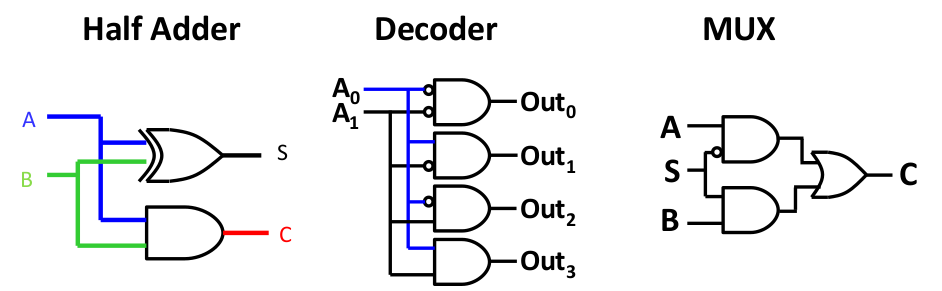
\includegraphics[scale=0.225]{combcircuits}
\begin{tabular}{@{}ll@{}}
\verb!Half Adder!    & basic gate of ALU \\
\verb!Decoder!  & basic gate of indexing \\
\verb!MUX!  & basic gate of data movement \\
\end{tabular} \\
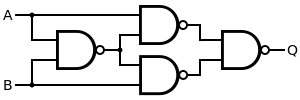
\includegraphics[scale=0.35]{XOR_NAND}
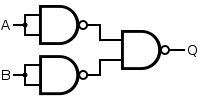
\includegraphics[scale=0.35]{OR_NAND}\\
XOR \ \ \ \ \ \ \ \ \ \ \ \ \ \ \ \ \ \ \ \ \ \ \ \ \ \ \ \ \ \ \ OR
\subsubsection{LC2K-ALU}
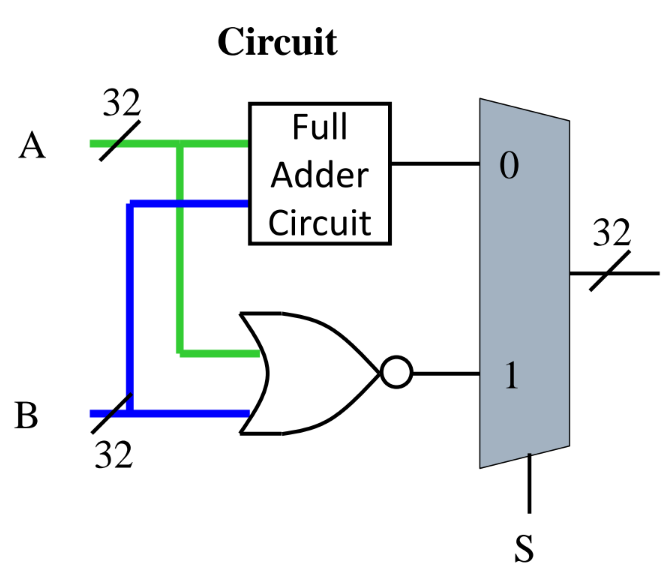
\includegraphics[scale=0.2]{LC2K-ALU}
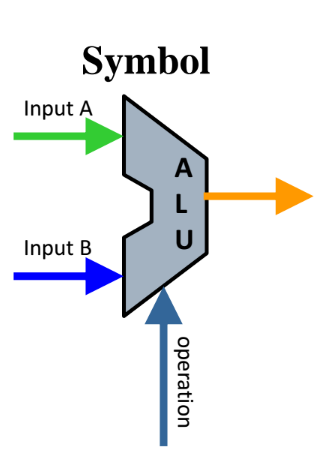
\includegraphics[scale=0.25]{LC2K-ALU2} \\
For LC2K, operation may either be add or nand.
\subsection{Sequential logic}
\subsubsection{Transparent D-latch}
$Q$ is set to $D$ only if gating signal ($G$) is 1, else the original value is maintained. 
In finite-state machines, think of $D$ as next state and $Q$ as current state.
\subsubsection{Edge triggered D flip-flop}
\begin{tabular}{@{}ll@{}}
\verb!positive edge!    & edge moving from 0 to 1 \\
\verb!negative edge!  & edge moving from 1 to 0 \\
\end{tabular} \\
Made using two d-latches, with direct/inverted clock signal going to two latches's gating signal. \\
\begin{tabular}{@{}ll@{}}
\verb!inverter on first latch!    & positive edge activated \\
\verb!inverter on second latch!  & negative edge activated \\
\end{tabular} \\
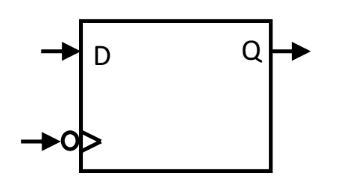
\includegraphics[scale=0.25]{flipflop}
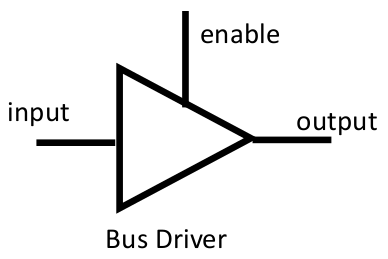
\includegraphics[scale=0.2]{tristate}
\subsubsection{Tri-state logic}
Three possible states: one, zero, not connected
\subsection{Finite state machine}
\begin{tabular}{@{}ll@{}}
$T(s,i)$  & current state \& input to output state \\
$P(s)$/$P(s,i)$  & current state to output \\
\end{tabular} \\
Types of FSM:
\begin{tabular}{@{}ll@{}}
Moore ($P(s)$)  & Output dependent on curr state \\
Mealy ($P(s,i)$)  & Output dependent on curr state \& input \\
\end{tabular} \\
\subsection{Single cycle processor design}
\begin{enumerate}
\item Fetch instructions
\item Decode instructions (Read data from ROM)
\item ROM output controls data movement (inc. PC, read registers, ALU control)
\end{enumerate}
Each instruction is one cycle, clock drives movement. Clock period is the time it takes to execute the slowest instruction.
\subsubsection{Clock speed example}
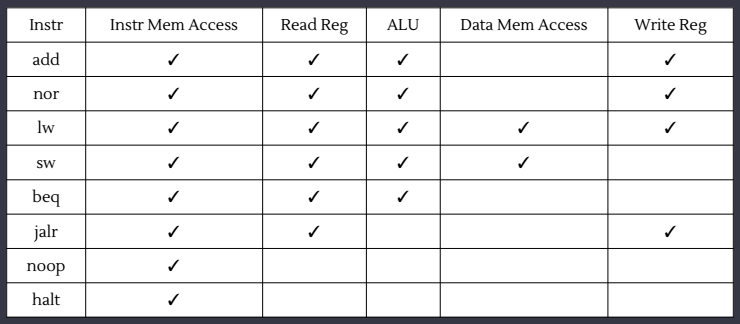
\includegraphics[scale=0.32]{instructions}
\begin{tabular}{|c|c|}
\hline
Read memory  & 4 ns \\
Write memory & 3 ns \\
Read register file & 5 ns \\
Write register file & 4.5 ns \\
ALU & 4.5 ns \\
Others & 0 ns \\
\hline
\end{tabular} \\
Then slowest instruction would be \verb!lw!, since
\begin{tabular}{|c|c|}
\hline
Read instruction  & 4 ns \\
Read \verb!regA! \& \verb!regB! & 5 ns \\
ALU \verb!regA! + \verb!offset! & 4.5 ns \\
Read resulting memory & 4 ns \\
Write \verb!regB! & 4.5 ns \\
\hline
Total & 22 ns \\
\hline
\end{tabular} \\
\subsubsection{Control building blocks}
\begin{tabular}{@{}ll@{}}
\verb!MUX!  & Select either one of input \\
\verb!Decoder!  & Map instruction to ROM address \\
\end{tabular} \\
\subsubsection{Compute building blocks}
\begin{tabular}{@{}ll@{}}
\verb!ALU!  & Basic arithmetic operations (ADD or NAND) \\
\verb!Sign extension!  & Repeats most significant bit to output size \\
  & OUT(31:0) = SE(IN(15:0)) \\
  & OUT(31:16) = IN(15) \\
  & OUT(15:0) = IN(15:0) \\
\end{tabular} \\
\subsubsection{State building blocks}
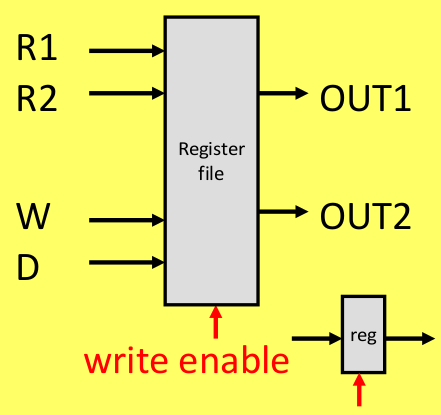
\includegraphics[scale=0.2]{register}
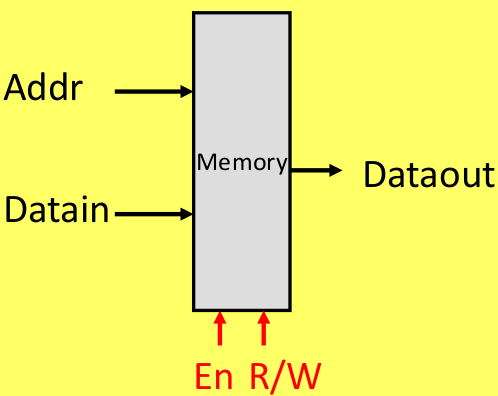
\includegraphics[scale=0.2]{memory}\\
R1, R2, W are 3 bits each, specify OUT1 \& OUT2.
\subsubsection{LC2K datapath example}
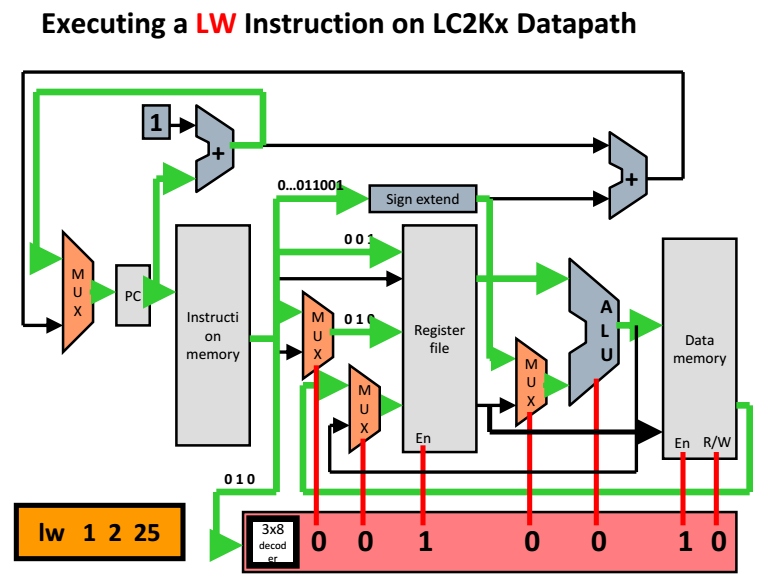
\includegraphics[scale=0.32]{lc2k-datapath-lw}

\subsection{Multi-cycle CPU}
\subsubsection{Multi-cycle datapath example}
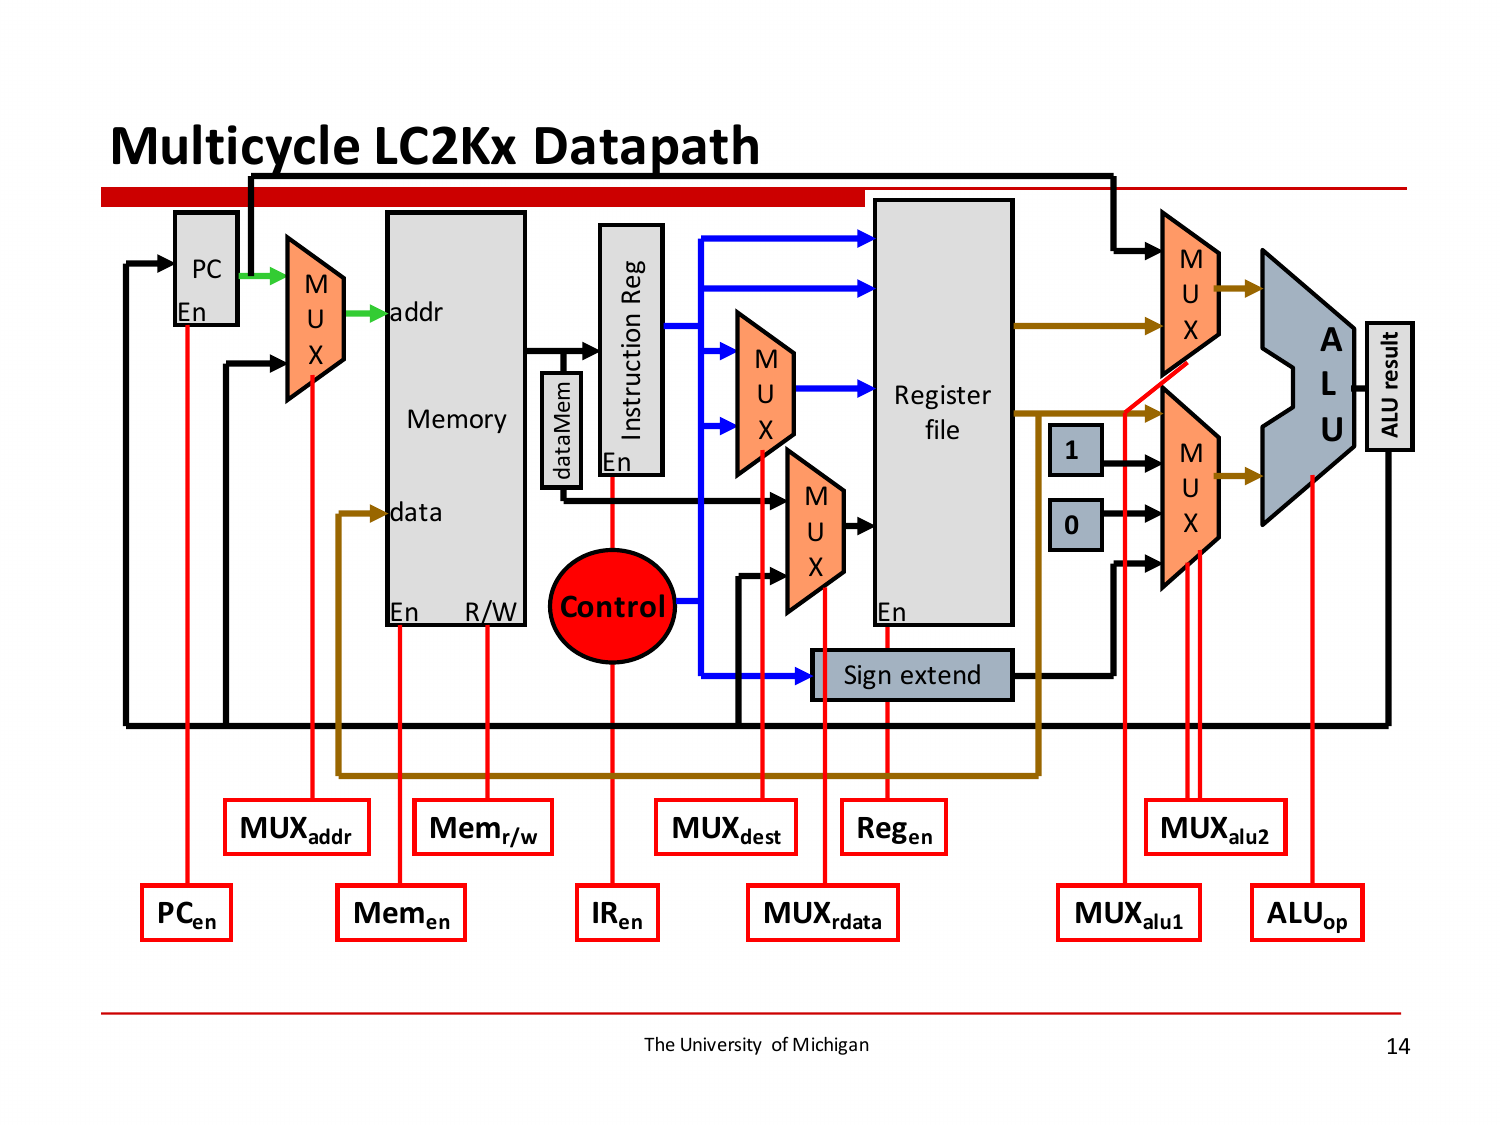
\includegraphics[scale=0.35]{multicycle_datapath}
\subsubsection{Multi-cycle FSM example}
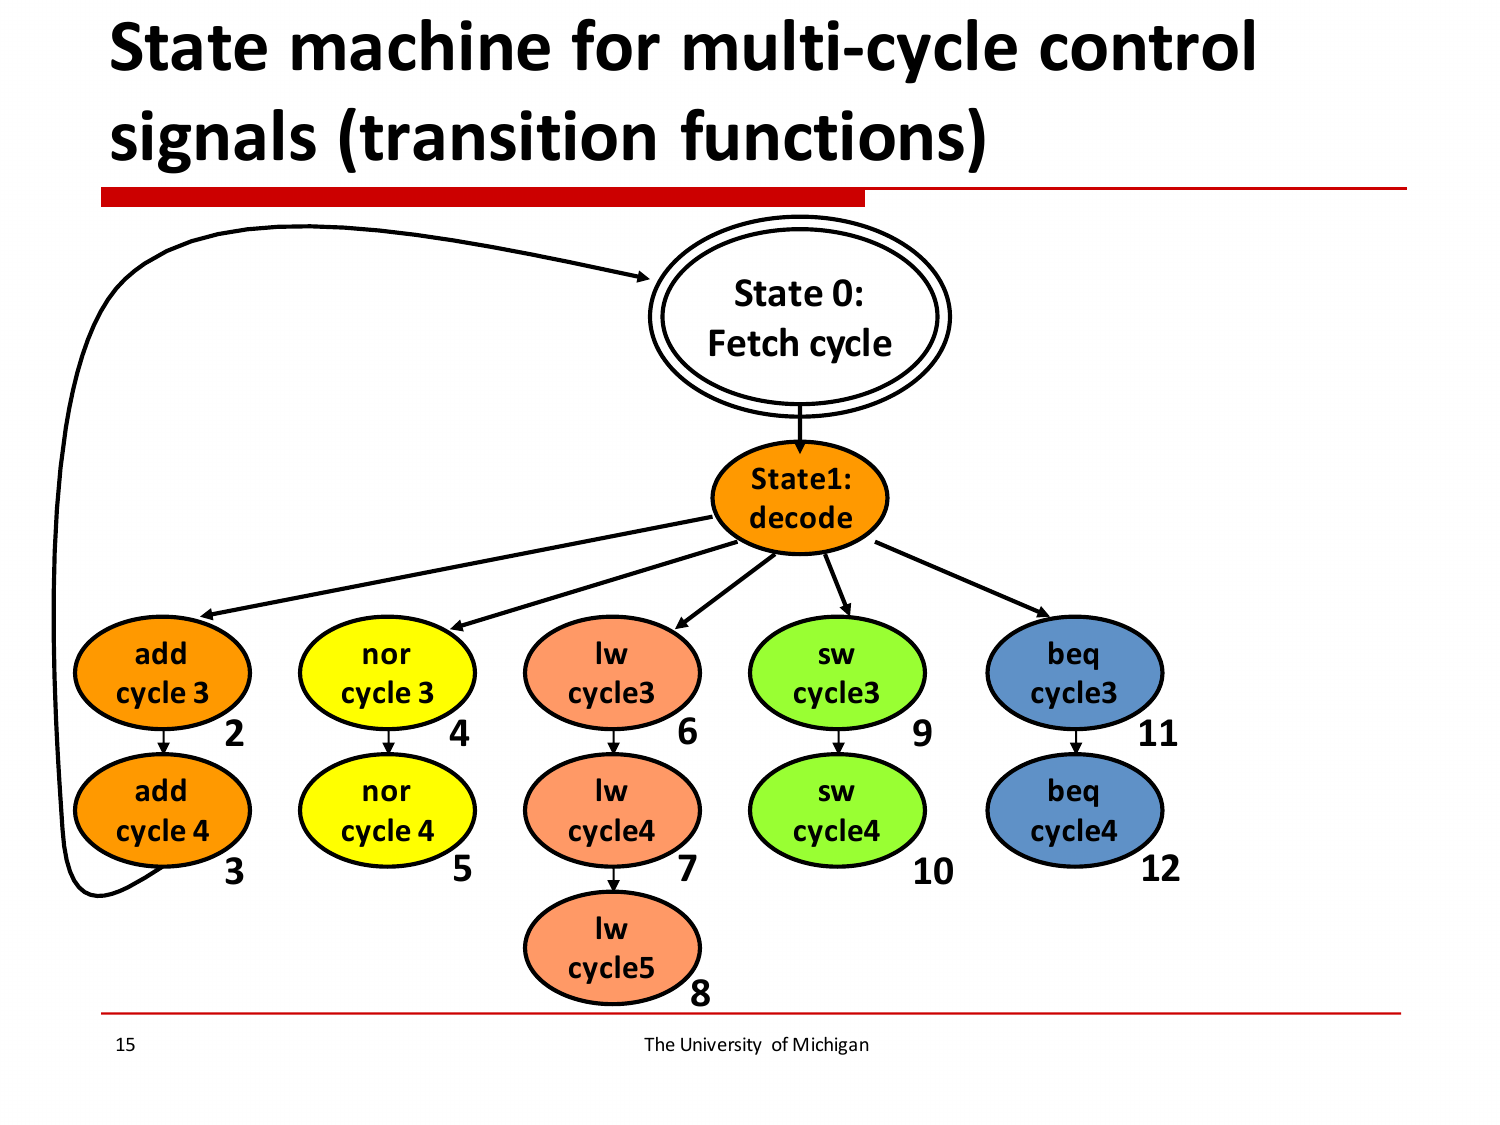
\includegraphics[scale=0.35]{multicycle_statemachine}
\subsubsection{FSM example}
\begin{enumerate}[start=0]
\item Fetch Cycle
  \begin{enumerate}
    \item mem[\verb!PC!] \textrightarrow \ instruction register
    \item Calculate \verb!PC! + 1
  \end{enumerate}
\item Decode
\item ALU
  \begin{enumerate}
    \item \verb!regA! + \verb!offset! for lw
    \item for beq, do equality check also
  \end{enumerate}
\item Read memory (Can store in a temporary data mem)
\item Write back (Write actual value to register)
\end{enumerate}
\subsubsection{Performance metrics}
\begin{itemize}
  \item Response time (Execution time)
  \begin{enumerate}
    \item Execution time = total instructions $\times$ CPI $\times$ clock period
    \item CPI = avg number of clock cycles per instruction for an application, For multicycle we need
    \begin{enumerate}
      \item Cycles necessary for each type of instruction
      \item Mix of instructions executed in the application
      \item Calculate new CPI from baseline CPI
    \end{enumerate}
  \end{enumerate}
  \item Throughput (work/time)
\end{itemize}

\subsection{Pipelining\ldots \ \emph{for dummies!}}
\subsubsection{Hazards}
\begin{itemize}
  \item Data: since register reads occur in stage 2 and
register writes occur in stage 5 it is possible to read the
wrong value if it is about to be written.
  \item Control: A branch instruction may change the PC,
but not until stage 4. What do we fetch before that?
  \item Exception: How do you handle exceptions in a pipelined
processor with 5 instructions in flight?
\end{itemize}

\subsubsection{Data hazards}
\begin{itemize}
  \item Avoid: Insert noops
    \begin{itemize}
      \item not portable
      \item large programs
      \item CPI is 1, but execution is slower due to noops
    \end{itemize}
  \begin{lstlisting}[language=Assembler]
  add   1   2   3   write 3 in cycle 5
  noop
  noop
  nand  3   4   5   read 3 in cycle 5
  \end{lstlisting}

  \item Detect \& Stall: CPI increases
    \begin{itemize}
      \item pass noop to execute
      \item stall at decode, if RaW dependency
    \end{itemize}

  \item Detect \& Forward: May still need stalling.
  \begin{lstlisting}[language=Assembler]
  lw  3   6   10    reg 6 at MEM stage
  sw  6   2   10    stall 1 cycle
  \end{lstlisting}
\end{itemize}

\subsubsection{Control hazards}
\begin{itemize}
  \item Avoid
    \begin{itemize}
      \item not portable
      \item large programs
      \item CPI is 1, but execution is slower due to noops
    \end{itemize}
  \item Detect \& Stall: CPI increases
    \begin{itemize}
      \item if opcode is branch, pass noop to decode
    \end{itemize}

  \item Speculate \& Squash
    \begin{itemize}
      \item assume not equal
      \item squash at write-back, draw table
      \item send noop to memory, execute, decode
      \item branch direction prediction using FSM
    \end{itemize}
\end{itemize}

\subsection{Cache Magic}
\begin{itemize}
  \item Temporal locality: if you access a memory location (e.g., 1000) you will be more likely to re-access that location than you will be to reference some other random location
  \item Spacial locality: if we reference a memory location (e.g., 1000), we are more likely to reference a location near it (e.g. 1001) than some random location
\end{itemize}
\subsubsection{Cache avg latency}
\begin{itemize}
  \item Avg access latency = cache latency $\times$ hit rate $+$ memory latency $\times$ miss rate
\end{itemize}
\begin{itemize}
  \item Cache: 1 cycles (90\% hit)
  \item Memory: 36 cycles (99\% hit)
  \item Disk: 400 cycles (100\% hit)
\end{itemize}
Latency: $1 + 0.1 \cdot (36 + 0.01 \cdot 400) = 5$

\subsubsection{Stores?}
\begin{itemize}
  \item In cache? Send it to cache.
  \begin{itemize}
    \item write-through: also send it to memory
    \item write-back: mark it dirty, write on evict
  \end{itemize}

  \item Not in cache? Write to memory
  \begin{itemize}
    \item allocate-on-write: bring the memory to cache first?
    \item no-allocate-on-write: don't do that
  \end{itemize}
\end{itemize}

\subsubsection{Mapping}
\begin{itemize}
  \item Fully-associative: Any memory location can be copied to any cache line.
  \item Direct-mapped: Memory block can go into specified cache block. Line index bit size is $\log_2(\textmd{\# of blocks})$
  \item Set-associative: Like directed-mapped but with fewer sets. Couple of blocks make a set. Set index bit size is $\log_2(\textmd{\#-way})$. \# sets = \#-lines / \#-ways
\end{itemize}

\subsubsection{Misses}
\begin{itemize}
  \item Compulsory: First reference to a block
  \item Capacity: Run out of space
  \item Conflict: Block is evicted
\end{itemize}
How? Three step process!
\begin{enumerate}
  \item Simulate cache with $\infty$ size \textrightarrow \ compulsory misses
  \item Fully-associative cache with intended size \textrightarrow \ any new misses capacity misses
  \item Actual cache \textrightarrow \ any new misses conflict misses
\end{enumerate}

\subsection{Virtual Memory}
Uses:
\begin{itemize}
  \item Multiple program can share memory without:
  \begin{itemize}
    \item transparency: know other programs exist
    \item protection: program only access its' memory
  \end{itemize}
\end{itemize}
\begin{itemize}
  \item Page fault: V pages misses, handled as exceptions
  \item Page table: virtual page \textrightarrow \ physical page, get physical address by physical page with offset
\end{itemize}

\subsubsection{Page table}
1GB = $2^{30}$ bytes of physical memory \& 4KB = $2^{12}$ page size, then the physical page number is 30-12 = 18 bits, plus another valid bit + other useful stuff (read only, dirty, etc.). Approx 3 bytes.
How can we organize it?
\begin{itemize}
  \item Continuous 3MB region of physical memory
  \item Use a multi-level page table! (Build a hierarchical page
table, keep in physical memory only the translations used)
  \begin{itemize}
    \item Super page table in physical memory
    \item Second (and maybe third) level page tables only if needed
    \item Size is proportional to the amount of memory used
    \item Example: Assuming size is 4KB 
    \begin{itemize}
      \item Min memory used: 4KB (Super page table)
      \item Max memory used: 4KB $+$ $1024 \cdot 4$KB
    \end{itemize}
  \end{itemize}
\end{itemize}
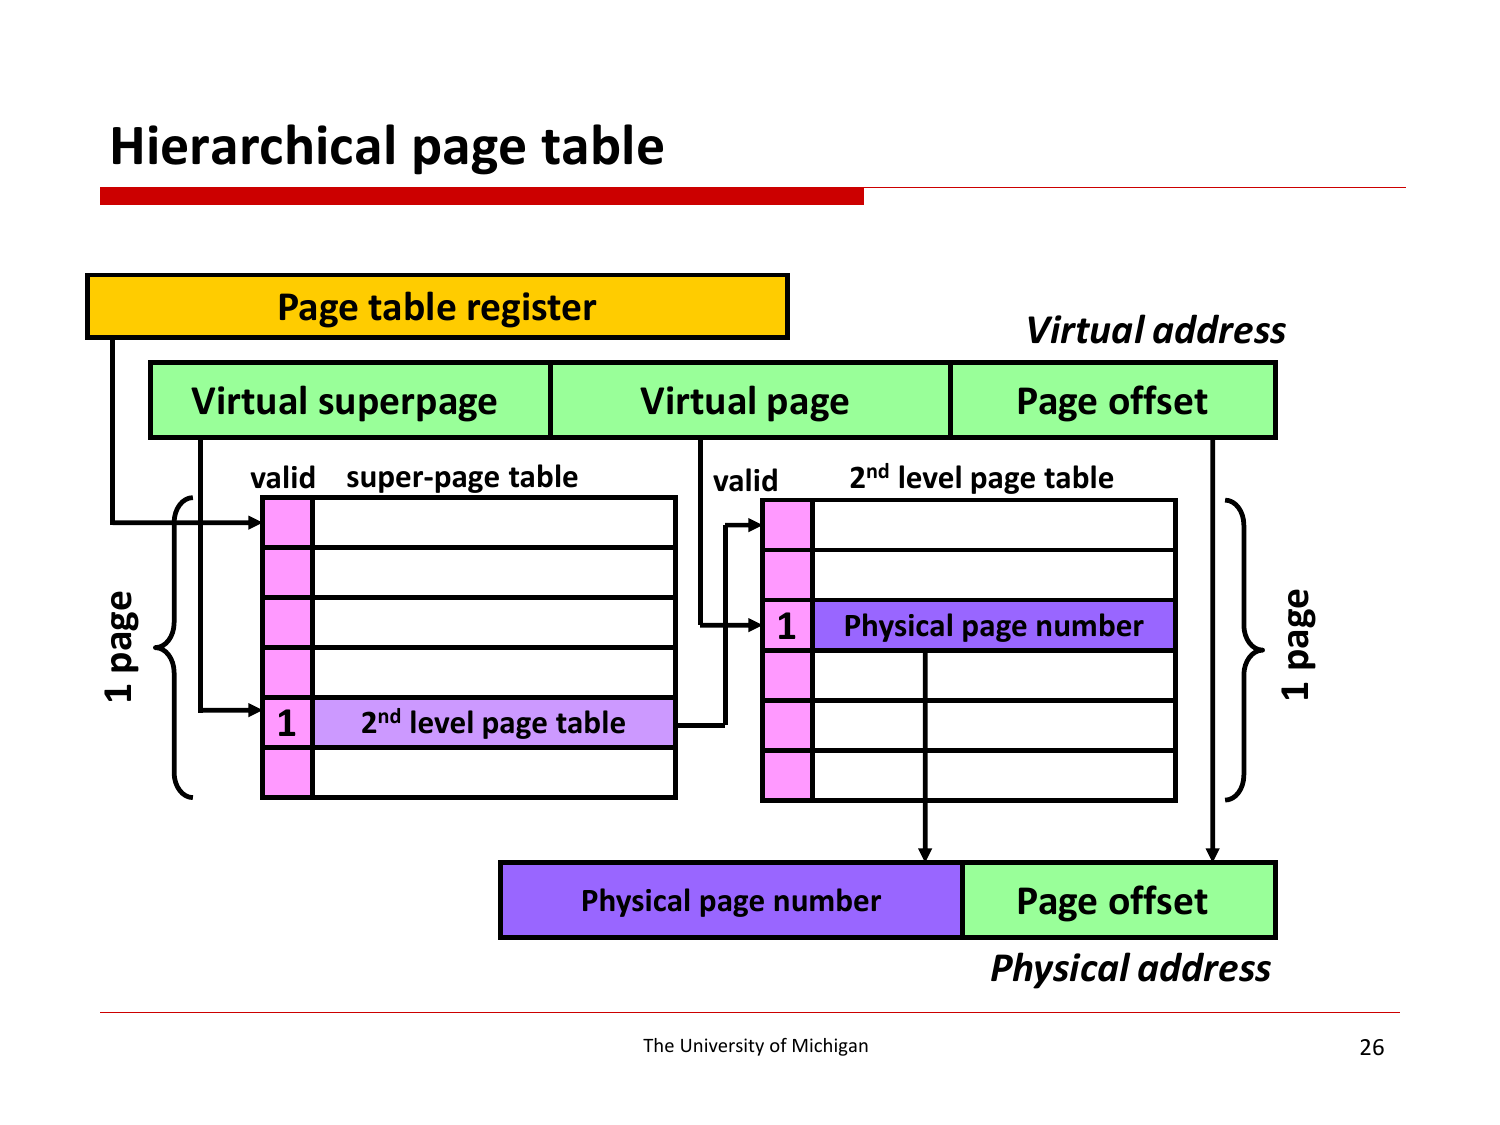
\includegraphics[scale=0.33]{ptable}

How can we replace it?
\begin{itemize}
  \item LRU: Reference bit on page, OS clears occasionally. Evict any “unreferenced” page.
\end{itemize}

\subsection{VM cache}
\begin{itemize}
  \item Virtual addr: Faster access? More complex?
  \item Physical addr: Delayed access? More complex?
\end{itemize}

\subsubsection{Translation look-aside buffer (TLB)}
\begin{itemize}
  \item Avoid main memory in virtual \textrightarrow \ physical addr translation (so it's fast)
\end{itemize}
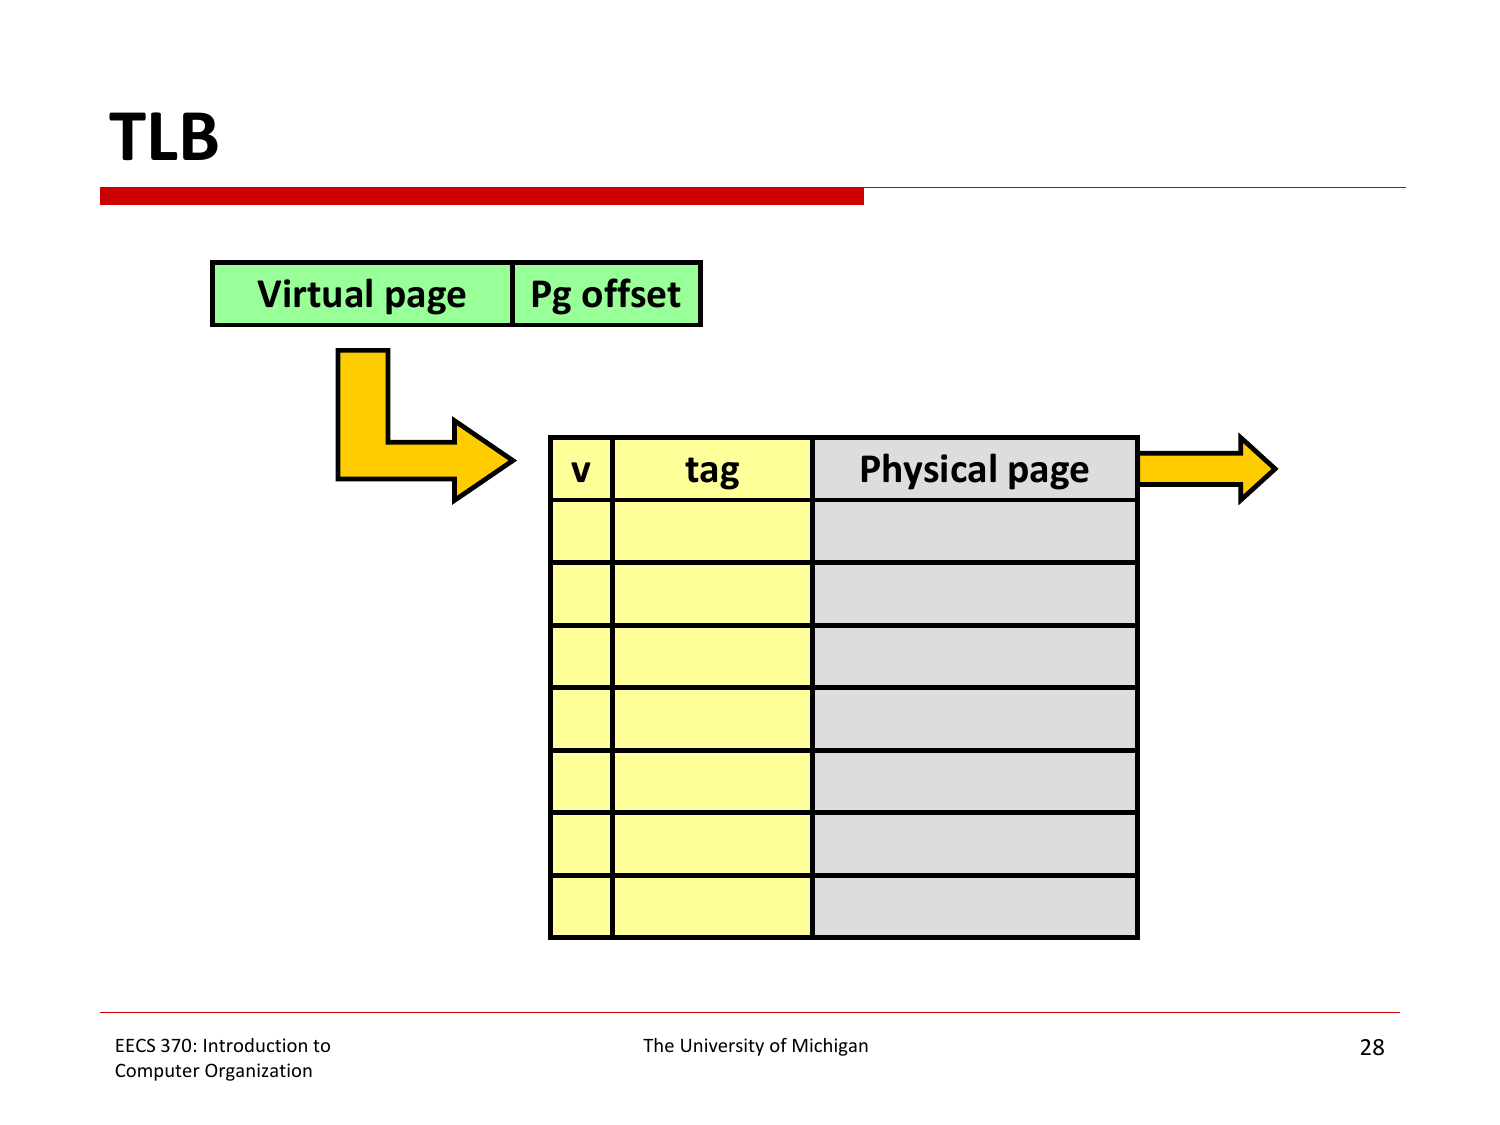
\includegraphics[scale=0.32]{tlb}
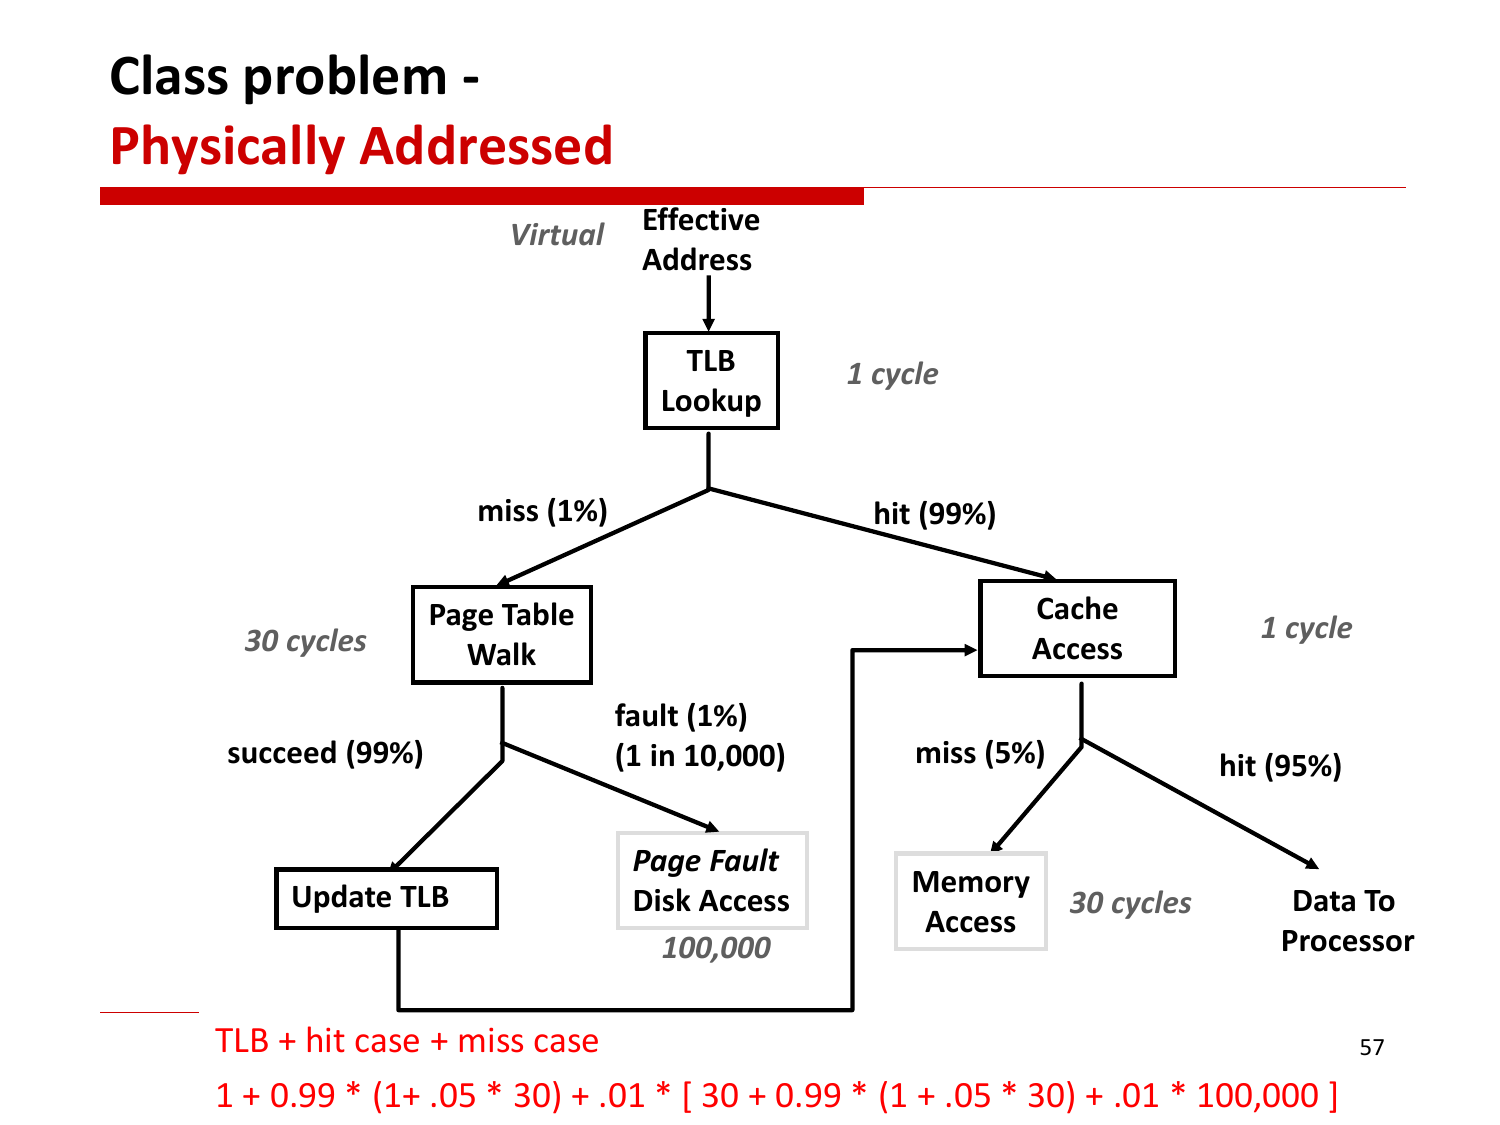
\includegraphics[scale=0.32]{physical_addr_map}
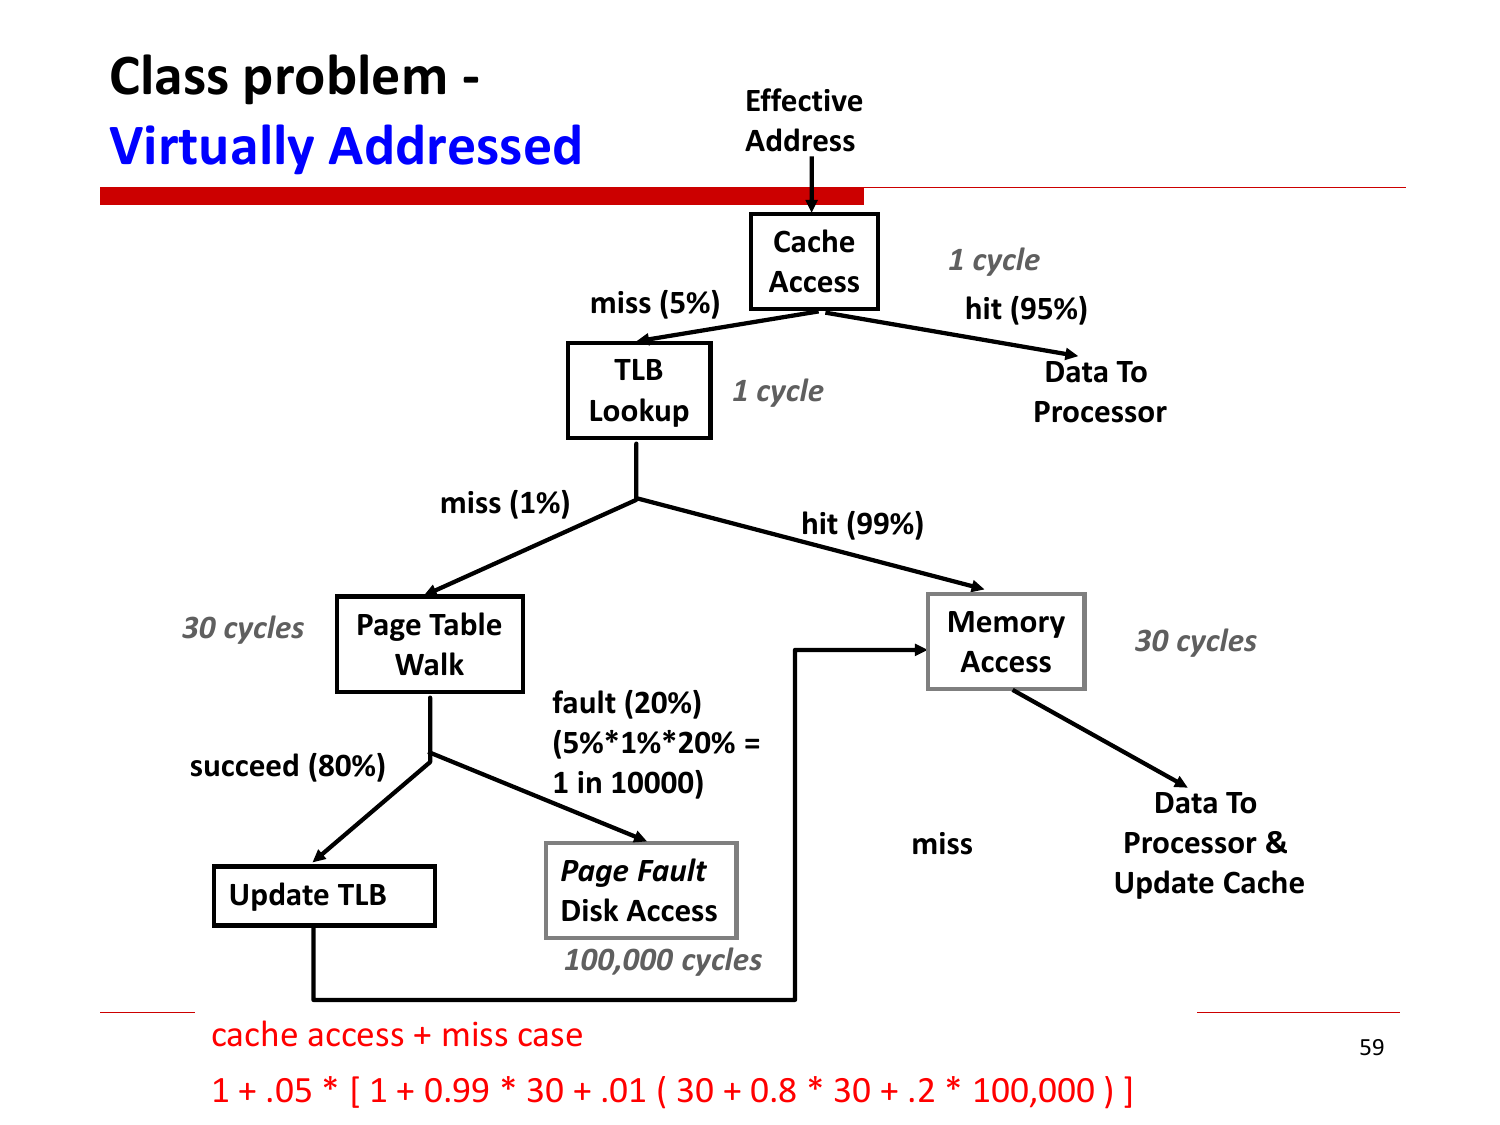
\includegraphics[scale=0.32]{virtual_addr_map}

\rule{0.3\linewidth}{0.25pt}
\scriptsize

bang your head against the wall

\end{multicols}
\end{document}
